En esta sección investigamos un enfoque distinto al de las secciones previas, en las cuales buscamos calcular todas las clases de equivalencia y sus representantes, para poder luego computar el $ASV$ de forma exacta. En cambio, ahora presentaremos un algoritmo probabilístico aproximado basado en la idea de samplear órdenes topológicos del DAG causal $G$.
Este nuevo algoritmo, a través de un mecanismo que pueda generar los órdenes topológicos de forma uniforme, busca estimar el valor de $ASV$ con una buena precisión, en base a la cantidad de muestras tomadas. De hecho, como veremos, la cantidad de sampleos necesarios crece lentamente con la precisión deseada, por lo que el método resulta eficiente. La formalización de esta idea se detalla en la sección \ref{subsubSection:proofErrorSamplingASV} del apéndice.

%\santi{Mandaría el lema al apéndice y contaría la idea. Es demasiado técnico para el flow que viene teniendo el resto del trabajo.}

El objetivo inicial consiste en devolver un orden topológico aleatorio para un DAG cualquiera. Nuestro primer acercamiento fue utilizar un algoritmo que genera todos los órdenes topológicos, en nuestro caso el algoritmo de Knuth \cite{algorithmForAllTopoSorts}, para luego ir devolviendo los órdenes mientras los generábamos. El problema que tiene este enfoque es que este proceso no es realmente aleatorio por varios motivos. Primero, siempre vamos a devolver los mismos y además en el mismo orden, pues el algoritmo de Knuth es determinístico. Además, no vamos a estar teniendo en cuenta la distribución de los mismos si el 99\% de los órdenes comienzan con los mismos nodos, entonces nos gustaría que eso se vea reflejado en nuestro sampleo, y en el caso de utilizar un algoritmo como el de Knuth, nos podría pasar que los órdenes que devolvamos sean muy poco probables. 

Otra alternativa es generar todos los órdenes y samplear uniformemente de los mismos. La dificultad radica en que generar todos los órdenes es demasiado costoso ($O(n!)$), y en el caso de generarlos, sería mejor agruparlos en las clases de equivalencias correspondientes y utilizar el algoritmo exacto, en vez de samplear de los mismos. Por lo tanto, esta idea tampoco resulta muy útil en la práctica. 

%\santi{Estos dos párrafos son raccontos de lo que fuimos pensando. Creo que no hace falta ponerlos. Al menos, reflexionaría sobre qué aporta dejarlos.} Reflexionamos y elegimos dejarlo Rta: Luego de una reflexión, banco dejarlos, aunque no sumen tanto muestran como se llegó a la idea

Así es como llegamos a nuestro algoritmo de sampleo, el cual depende de poder contar la cantidad de órdenes de un DAG para poder samplear correctamente.  

\subsection{Algoritmo de sampleo}

Para dar una intuición de este algoritmo vamos a utilizar la Figura \ref{fig:topoSortSamplingExample}. Este es un grafo con 600 órdenes topológicos, 100 de estos comienzan con $source_1$, 300 con $source_2$ y 200 con $source_3$. Definimos a $S$ como el conjunto de nuestros nodos fuente (source nodes). Teniendo en cuenta lo mencionado previamente, querríamos que el orden que sampleemos tenga una probabilidad mayor de comenzar con $source_2$ que con los otros dos nodos fuente, ya que hay una mayor cantidad de órdenes que comienzan con ese nodo. Nuestro algoritmo utiliza esta idea para obtener un orden topológico. Primero, según la cantidad de órdenes topológicos que comienzan con cada uno, define una distribución para cada nodo, que asigna una probabilidad proporcional a la cantidad de órdenes topológicos que comienzan con ese nodo. Luego vamos a elegir nuestro siguiente nodo del orden en base a esa distribución, y por último vamos a remover del grafo nuestro nodo elegido, para seguir generando el orden recursivamente a partir de los nodos restantes. 
%\echu{Poner explicitamente cual es la distribución, osea que es una distribución proporcional a la cantidad de ordenes topológicos con los que empieza }

%\santi{Excelente dibujo}

\begin{figure}[ht]
    \centering
    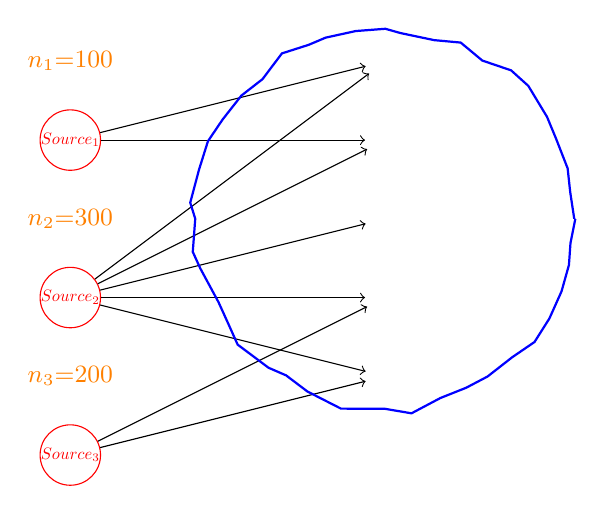
\begin{tikzpicture}
        % Define the rigth set of nodes
        \foreach \i in {1,2,3,4,5}
            \node[draw=none, circle, minimum size=5mm, inner sep=0pt] (L\i) at (4, -\i) {};

        % Define the left set of nodes
        \foreach \j in {1,2,3}
            \node[draw, circle, red, minimum size=5mm, inner sep=0pt] (source\j) at (0, -\j*2) {\scalebox{0.6}{$Source_\j$}};

        % Draw edges between nodes (example edges)
        \foreach \i in {1,2}
            \foreach \j in {1,2}
                \draw[->]  (source\j) -- (L\i); 

        \foreach \i in {4,5}
            \foreach \j in {2,3}
                \draw[->]  (source\j) -- (L\i); 

        \draw[->]  (source2) -- (L3);
        

         \draw [decorate, blue, decoration={random steps, segment length=10pt, amplitude=2pt}, thick]
        (4,-3) circle (2.4);

        %Number of órdenes topológicos for each node

        \node[draw=none,minimum size=3mm, inner sep=0pt] () at (0, -1) {\small \textcolor{orange}{$n_1$=100}};

        \node[draw=none,minimum size=3mm, inner sep=0pt] () at (0, -3) {\small \textcolor{orange}{$n_2$=300}};

        \node[draw=none,minimum size=3mm, inner sep=0pt] () at (0, -5) {\small \textcolor{orange}{$n_3$=200}};
    \end{tikzpicture}
    \caption{Posible comienzo del algoritmo de sampleo, con los candidatos a ser el primer nodo del orden en rojo y el resto del grafo en azul. Cada node fuente (source) tiene sus respectivas cantidades de órdenes topológicos en los que está primero.}
    \label{fig:topoSortSamplingExample}
\end{figure}

\begin{algorithm}
\caption{SampleoTopoSort($D$)} \label{alg:topoSortSampling}
\begin{enumerate}
    \item \textbf{Calculamos una probabilidad} $p$ para cada uno de los nodos fuente del DAG.
        \begin{enumerate}
            \item Para cada $s \in S$ lo removemos del DAG $D$, y contamos la cantidad de órdenes topológicos en $D-\set{s}$ ($toposorts_s$), este valor es la cantidad de órdenes que comienzan con $s$.
            \item Luego a cada $s \in S$ le asignamos una probabilidad $p(s)= \frac{toposorts_s}{\#topos(D)}$. 
        \end{enumerate}
    \item \textbf{Sampleamos} sobre $S$ utilizando $p$ para obtener nuestro primer nodo $start$.
    \item \textbf{Eliminamos} a $start$ de $D$ y llamamos al algoritmo recursivamente con  SampleoTopoSort($D-\set{start}$), guardando el resultado en $orden$. 
    \item \textbf{Devolvemos} $start + orden$ como el orden topológico sampleado. 
\end{enumerate}
\end{algorithm}

%\echu{ Agrego el algoritmo en pseudocodigo o no hace falta?}
%\santi{El que está ahora me parece excelente.}

En la implementación de este algoritmo\footnote{Pueden encontrar este algoritmo en \path{\pasantia-BICC\asvFormula\topoSorts\randomTopoSortsGeneration.py}} también utilizamos una caché para el número de órdenes topológicos de cada subgrafo del DAG, de esta forma nos ahorramos calcular más de una vez el conteo de los órdenes para un mismo subgrafo.

Para nuestro caso de uso vamos a necesitar más de un orden, ya que necesitamos samplear varios órdenes. Por lo que ahora nuestra función va a ser \texttt{SampleoTopoSorts}($D$, $k$), la cual recibe $k$ además de $D$, y devuelve $k$ órdenes topológicos aleatorios del DAG $D$. La implementación naive de esta función sería llamar $k$ veces a \texttt{SampleoTopoSorts}. Pero si hacemos esto vamos a estar repitiendo varias veces los mismos pasos, cuando los podríamos hacer en simultáneo. Vamos a calcular $k$ veces la probabilidad $p$ para los nodos fuente de $D$, y eliminaremos $k$ veces cada nodo elegido de $D$. En cambio, una alternativa mejor consiste en calcular una vez $p$ y obtener los $k$ nodos necesarios para cada iteración. 
Por lo tanto, hay que realizar dos modificaciones a nuestro Algoritmo \ref{alg:topoSortSampling} para no realizar estas operaciones innecesariamente. En  el paso $2$, vamos a samplear $k$ nodos de $S$ (puede haber nodos repetidos). Esto nos va a devolver un número $k_s$ para cada $s \in S$ ($\sum_{s \in S} k_s = k$), que es la cantidad de órdenes que van a comenzar con ese nodo. Luego vamos a llamar a \texttt{SampleoTopoSorts}($D-{s}$, $k_s$) para cada $s$ con $k_s > 0$, y agregar $s$ al comienzo de cada uno de los $k_s$ órdenes obtenidos. 

%\echu{ Misma duda que arriba, agrego el algoritmo en pseudocodigo/palabras o no hace falta?}
%\santi{Capaz podés poner el pseudocódigo del más complicado y listo (que es aparte el que usamos, no?)}
%\echu{Releyendolo creo que no hace falta, pero no se. Me parece que queda más lindo dejar el pseudocodigo del más simple que se entiende bonito} Cifu: Queda bien, no hace falta el pseudocódigo.

\subsection{Número de órdenes topológicos de un polytree}

\begin{figure}[ht]
\centering 
 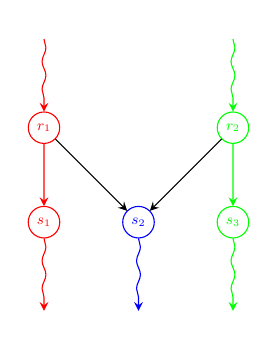
\begin{tikzpicture}[scale=.60, transform shape]
        % ---- NODOS ----
        \node[nodo, red] (r1) at (-2,0) {$r_1$};

        \node[nodo, green] (r2) at  (2,0) {$r_2$};
        
        \node[nodo, red] (s1) at (-2,-2) {$s_1$};
        \node[nodo, blue] (s2) at (0,-2) {$s_2$};
        \node[nodo, green] (s3) at (2,-2) {$s_3$};
        

        \node[draw=none, fill=none] (h1) at (-2, -4) {};
        \node[draw=none, fill=none] (h1Parent) at (-2, 2) {};
        \node[draw=none, fill=none] (h2) at (0, -4) {};
        \node[draw=none, fill=none] (h3) at (2, -4) {};
        \node[draw=none, fill=none] (h3Parent) at (2, 2) {};


         \path [->] (r1) edge[arista, red]  (s1);
         \path [->] (r1) edge[arista]  (s2);
         \path [->] (r2) edge[arista]  (s2);
         \path [->] (r2) edge[arista, green]  (s3);

        \path [->] (s1) edge[arista, red, mySnake] (h1);
        \path [->] (h1Parent) edge[arista, red, mySnake] (r1);
         \path [->] (s2) edge[arista, blue,  mySnake]  (h2);
         \path [->] (s3) edge[arista, green,  mySnake]  (h3);
         \path [->] (h3Parent) edge[arista, green,  mySnake]  (r2);

    \end{tikzpicture}
    \caption{Ejemplo de polytree para el cual no funciona la Fórmula \ref{for:topoCountingDTrees}, la cual cuenta los órdenes topológicos de un \dtree. Los descendientes en común y disjuntos de cada raíz están marcados de un color distinto.}
    \label{fig:notWorkingDtreeColored}
\end{figure}
%\echu{ Entiendo que está mal decirle subarbol, como le digo sino? Le invento un nombre? }

Para poder utilizar este algoritmo de sampleo necesitamos poder contar el número de órdenes topológicos de nuestro DAG. Actualmente, ya podemos contar los órdenes de un \dtree{}, pero nuestro objetivo era poder tratar con una familia de grafos más amplia, por lo que vamos a volver al ejemplo para el cual la Fórmula \ref{for:topoCountingDTrees} no podía contabilizar correctamente el número de órdenes topológicos. En la Figura \ref{fig:notWorkingDtreeColored} no podemos usar la misma estrategia que para el árbol, puesto que hay un solapamiento entre los subárboles de $r_1$ y $r_2$, todos los descendientes de $s_2$. A partir de esto, el caso que queremos resolver es cuándo un nodo tiene dos o más padres. Para resolver este problema, comenzamos con un enfoque similar al realizado en el Algoritmo \ref{for:topoCountingDTrees} para \dtrees, pero nos encontramos con un caso para el cual no funcionaba. Luego terminamos cambiando el enfoque y llegamos a un nuevo algoritmo, el cual nos permitió calcular todos los órdenes topológicos de cualquier polytree.   

\subsubsection{Idea inicial}

Nuestra idea para el resolver el caso de la Figura \ref{fig:notWorkingDtreeColored} consiste en calcular los resultados de los subárboles de $r_1,s_2$ y  $r_2$ por separado, para luego unificar sus resultados. En la Figura \ref{fig:multiples_toposorts_polytree} tenemos 3 órdenes posibles. Nuestro objetivo es combinarlos en un orden $\toOr$. Las únicas restricciones que tenemos que tener en cuenta al combinarlos es que $\toOr(s_2) < \toOr(r_1) \land \toOr(s_2) < \toOr(r_2)$, ya que $s_2$ es un descendiente de ambos nodos. 

 \begin{figure}[ht]
    \centering
    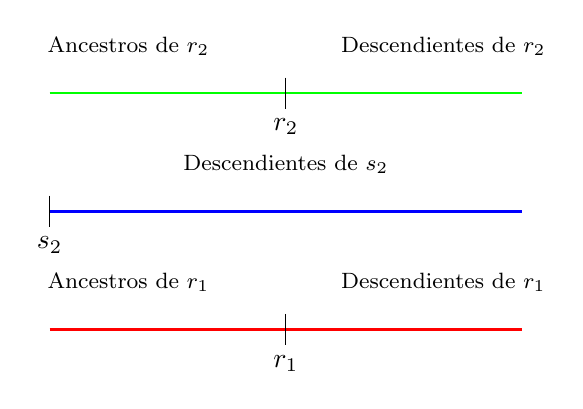
\begin{tikzpicture}

\foreach \y/\label/\color/\ancestor/\descendant in {
    0/$r_1$/red/{Ancestros de $r_1$}/{Descendientes de $r_1$}, 
    1.5/$s_2$/blue/{}/{}, 
    3/$r_2$/green/{Ancestros de $r_2$}/{Descendientes de $r_2$}} {  
    
    % Línea horizontal principal
    \draw[thick, color=\color] (1,\y) -- (7,\y);
    
    \pgfmathsetmacro{\yminus}{\y-0.2}
    \pgfmathsetmacro{\yplus}{\y+0.2}
    \pgfmathsetmacro{\ytext}{\y+0.6}
    
    % Etiquetas en vez de puntos suspensivos
    \node at (2,\ytext) {\footnotesize \ancestor};
    \node at (6,\ytext) {\footnotesize \descendant};

    % Posición del nodo raíz
    \pgfmathparse{\y == 1.5 ? 1 : 4} % s_2 a la izquierda, otros al medio
    \let\nodePosi\pgfmathresult
    
    % Ticks y etiquetas
    \draw (\nodePosi,\yplus) -- (\nodePosi,\yminus); 
    \node[below] at (\nodePosi,\yminus) {\label};
}

    \node at (4, 2.1) {\footnotesize Descendientes de $s_2$};
    \end{tikzpicture}
    \caption{Estos serían tres órdenes topológicos posibles, uno para cada subárbol de la Figura \ref{fig:notWorkingDtreeColored}. $s_2$ es la raíz de su subárbol, por lo que siempre va a estar primero.}
    \label{fig:multiples_toposorts_polytree}
\end{figure}

%\echu{El dibujo es medio pobre, agregarle algo a los puntitos suspensivos. En vez de poner esos puntos poner que unos son los "ancestros de $r_i$" y los otros son los "descendientes de $r_i$" o algo así, darle más sabor!}

Sabemos que estos 3 conjuntos de nodos no van a tener otras aristas que los conecten, ya que en ese caso no sería un polytree, pues se generaría un ciclo en el grafo subyacente. Por esto podemos combinar sus órdenes sabiendo que no va a haber solapamiento. De esta forma, nuestro algoritmo va a consistir en remover las aristas de los nodos que tienen múltiples padres, calcular el resultado para cada uno de sus subárboles y luego combinar estos resultados para obtener todos los órdenes. 

Nuestro primer intento se basó en utilizar el multinomial para combinar los órdenes, pero el problema de esta fórmula es que no tiene en cuenta la restricción pedida, que $r_1$ y $r_2$ aparezcan previamente a $s_2$. Otra opción sería combinar todos los órdenes de $r_1$ y $r_2$ para luego insertar los órdenes de $s_2$. Pero nos volvemos a encontrar con el mismo problema si combinamos los órdenes de $r_1$ y $r_2$ utilizando el multinomial, nos vamos a perder la información de dónde se encuentran estos dos nodos, y por lo tanto a partir de qué posición podemos colocar a $s_2$. Así es como llegamos a la conclusión de que necesitábamos calcular no solo la cantidad de órdenes topológicos y el tamaño de cada subárbol, sino que también debíamos guardarnos la posición de los padres $r_i$ en cada uno de esos órdenes. 

Para eso hicimos la función \texttt{positionInTopsorts}($D$, $n$)(o $pit)$, que dado un \dtree{} $D$ y un nodo $n$, retorna un conjunto $toposPositions$, el cual contiene duplas de la forma $(position, toposorts) \in toposPositions$, siendo $toposorts$ la cantidad de órdenes topológicos del \dtree{} $D$, en los cuales el nodo $n$ se encuentra en la posición $position$. Para nuestro ejemplo tenemos que calcular $positionInToposorts$ para los tres conjuntos de nodos marcados.

Vamos a definir a $\intersectionNode$ como nuestro nodo con más de un padre, en nuestro ejemplo sería $s_2$. Ahora queremos ver cómo combinar los resultados obtenidos al evaluar $positionInToposorts$ sobre cada uno de los padres e $\intersectionNode$\footnote{Cuando evaluamos $positionInToposorts(D-\set{(n,\intersectionNode)},p)$ con $p \in parents(\intersectionNode)$, removemos la arista que conecta $p$ a $\intersectionNode$ puesto que si no estaríamos calculando dos veces lo mismo, ya que vamos a correr $positionInToposorts(D,\intersectionNode)$.}. Como los padres no tienen ninguna restricción entre sí, pueden aparecer en cualquier orden. Luego, para cada uno de esos ordenamientos posibles, buscamos cuántos órdenes topológicos hay que respeten ese ordenamiento. Para calcular eso vamos a utilizar una función similar a la vista en el Algoritmo \ref{alg:leftOrdersAlgorithm}, llamaremos a esta función modificada $allPosibleOrders(before,after,parents, topos)$\footnote{Pueden encontrar este algoritmo en \path{\pasantia-BICC\asvFormula\topoSorts\topoSortsCalc.py}} (o $apo$). Esta función nos va a devolver todos los órdenes topológicos dado un ordenamiento de los padres y una lista de duplas $(pos,topo)$ (el output de $positionInTopsorts$) para cada padre. A diferencia de \leftPossibleOrders, los nodos que vamos a colocar no son los ancestros de $x_i$, sino los padres de $\intersectionNode$. Otra diferencia es que además de tener los nodos a la izquierda de los padres, también vamos a tener los nodos a la derecha para colocar. Los nodos a la izquierda de cada padre los obtenemos con su posición y los nodos a la derecha utilizando su posición y el tamaño del subárbol del padre.

%\echu{¿Hace falta una explicación más detallada de cómo funciona allPosibleOrders? Para mi no, pero es clave y después lo uso también} Rta: Cómo Cifu no lo marcó entiendo que no

Así llegamos a la función que nos va a permitir calcular los órdenes topológicos aunque haya más de un padre. Lo que vamos a hacer es iterar por todos los ordenamientos de los padres y luego iterar por todas las combinaciones posibles del output de $positionInToposorts$. Los parámetros de la función son:

\begin{itemize}
    \item $\intersectionNode$ : el nodo intersección.
    \item $ps$ : los padres de $\intersectionNode$. 
    \item $poly$ : el polytree que contiene los subárboles $\subtree_p$ para cada $p \in ps$. 
\end{itemize}

\begin{align}\label{formula:combineMultipleParents} 
    ordersFromIntersection(\intersectionNode, ps, poly) =&
    \sum_{p \in perm(ps)} \\& \nonumber
    \sum_{\substack{
    topos \in \\
    pit(p[1], \subtree_{p[1]}) \times \cdots \times pit(p[|p|], \subtree_{p[|p|]}) \times pit(\intersectionNode, \subtree_{\intersectionNode})
}}  apo(topos)
\end{align}

Así llegamos a la versión inicial de nuestro algoritmo. Primero recorremos el polytree en \newline \texttt{intersectionNodes} para obtener los distintos nodos con más de un padre. Luego para cada intersección utilizamos \newline \texttt{ordersFromIntersection} para obtener todos los órdenes. Por último, combinamos los resultados obtenidos para cada polytree al igual que con los \dtrees{}, ya que no hay aristas entre los distintos polytree por lo que no hay restricciones al combinarlos. La versión inicial del algoritmo\footnote{Pueden encontrar este algoritmo en \path{\pasantia-BICC\asvFormula\topoSorts\topoSortsCalc_basic.py}}: 

\begin{algorithm}
\caption{Versión inicial - Número de órdenes topológicos en polytrees} \label{alg:numberToposortsPolytreeFailed}
\begin{algorithmic}[1]
\Function{allPolyTopoSorts}{$polyTree$}
    \State $intersectionNodes \gets$ \Call{intersectionNodes}{$polyTree$}
    \State $topos \gets \set{}$
    \State $sizes \gets \set{}$

    \For{$inter \in intersectionNodes$}
        \State $topos \gets topos \ \cup $ \Call{ordersFromIntersection}{$inter, parents(inter), polytree$}
        \State $sizes \gets sizes \ \cup$ \Call{totalSize}{$polytree, inter$}
    \EndFor

    \State $totalToposorts \gets$ \Call{multinomialCoefficients}{$treeSizes$}
    \State $totalToposorts \gets totalToposorts \cdot \prod_{t \in topos} t$
    \State \Return $totalToposorts$
\EndFunction
\end{algorithmic}
\end{algorithm}


Ahora podemos resolver el caso de la Figura \ref{fig:notWorkingDtreeColored}, y más general aún, podemos resolver cualquier DAG que sea un polyforest que tenga sólo un nodo con múltiples padres en cada uno de sus polytrees. ¿Qué ocurre si tenemos más de una intersección como en la Figura \ref{fig:polytreeMultipleIntersections}? 

\begin{figure}[ht]
\centering 
 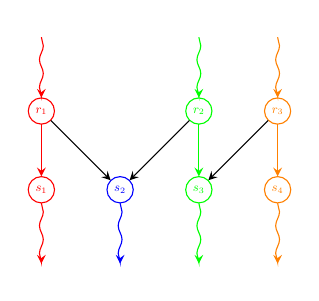
\begin{tikzpicture}[scale=.50, transform shape]

        % ---- NODOS ----
        \node[nodo, red] (r1) at (-2,0) {$r_1$};
        \node[nodo, green] (r2) at  (2,0) {$r_2$};
        \node[nodo, orange] (r3) at  (4,0) {$r_3$};
        
        \node[nodo, red] (s1) at (-2,-2) {$s_1$};
        \node[nodo, blue] (s2) at (0,-2) {$s_2$};
        \node[nodo, green] (s3) at (2,-2) {$s_3$};
        \node[nodo, orange] (s4) at (4,-2) {$s_4$};
        

        \node[draw=none, fill=none] (h1) at (-2, -4) {};
        \node[draw=none, fill=none] (h1Parent) at (-2, 2) {};
        \node[draw=none, fill=none] (h2) at (0, -4) {};
        \node[draw=none, fill=none] (h3) at (2, -4) {};
        \node[draw=none, fill=none] (h3Parent) at (2, 2) {};
        \node[draw=none, fill=none] (h4) at (4, -4) {};
        \node[draw=none, fill=none] (h4Parent) at (4, 2) {};


         \path [->] (r1) edge[arista, red]  (s1);
         \path [->] (r1) edge[arista]  (s2);
         \path [->] (r2) edge[arista]  (s2);
         \path [->] (r2) edge[arista, green]  (s3);
         \path [->] (r3) edge[arista]  (s3);
         \path [->] (r3) edge[arista, orange]  (s4);

        \path [->] (s1) edge[arista, red, mySnake] (h1);
        \path [->] (h1Parent) edge[arista, red, mySnake] (r1);
         \path [->] (s2) edge[arista, blue,  mySnake]  (h2);
         \path [->] (s3) edge[arista, green,  mySnake]  (h3);
         \path [->] (h3Parent) edge[arista, green,  mySnake]  (r2);
         \path [->] (s4) edge[arista, orange,  mySnake]  (h4);
         \path [->] (h4Parent) edge[arista, orange,  mySnake]  (r3);

    \end{tikzpicture}
    \caption{Ejemplo de polytree para el cual no funciona el algoritmo \ref{alg:numberToposortsPolytreeFailed} para contar los órdenes topológicos en polyforests. Cada subárbol que vamos a tener en cuenta está marcado de un color distinto.}
    \label{fig:polytreeMultipleIntersections}
\end{figure}

El problema yace en que para poder utilizar $ordersFromIntersection$, necesitamos poder aplicar \texttt{positionInTopsorts} sobre cada uno de los subárboles y que estos sean \dtrees. Pero sin importar si comenzamos por los padres de cualquiera de nuestras intersecciones ($s_2$ y $s_4$), vamos a tener un subárbol el cual no es un \dtree. Al no poder solucionar este caso a través de este primer enfoque, repensamos el algoritmo desde cero, buscando un enfoque distinto. A continuación veamos el algoritmo que surgió de este cambio, el cual terminó siendo el algoritmo para el caso general. 

%\echu{ ¿Tiene sentido que entre en más/menos detalle de esta idea que fue fallida? ¿Describo los algoritmos positionsInToposorts y allPolyTopoSortsOld? ¿O meramente cuento las ideas por arriba y muestro el caso para el cuál ya no funcionaba? Echu del futuro: Siento que ahí está bien, creo que no tiene sentido meterme mucho más en esto} Cifu: Confirmamos, no hace falta profundizar más

\subsubsection{Algoritmo final}

La idea surge de ver cómo calcular los órdenes desde un nodo, teniendo en cuenta que ya tenemos calculados los de todos los vecinos. Sabiendo lo que necesitamos para combinarlos, la posición de los vecinos, los órdenes y el tamaño de los subárboles, solo queda ver cómo unirlos. El algoritmo consiste en realizar un $DFS$ sobre el grafo subyacente del polytree para obtener sus órdenes topológicos. La función \texttt{polytreeToposorts}($node$, $D$) (o $polyTopo$) \footnote{Pueden encontrar este algoritmo en \path{\pasantia-BICC\asvFormula\topoSorts\topoSortsCalc.py}} va a retornar el mismo resultado que \texttt{positionInTopsorts}, dado un polytree $D$ y un nodo $node$ devuelve el conjunto $toposPositions$ para ese nodo (solo que esta función no necesita que $D$ sea un \dtree). Por ejemplo, en la Figura \ref{fig:dfsTopoSorts} comenzamos por $r_i$ revisando sus vecinos. Por ejemplo, al llegar a $d_3$, vamos a obtener sus vecinos \emph{no visitados} para calcular sus órdenes, al no tener ninguno vamos a devolver el conjunto $\set{(0,1)}$, ya que solo tiene un orden y se encuentra primero en ese orden. Este es nuestro caso base. Ahora queda ver el caso en el cual tenemos vecinos que no fueron visitados. 
%\santi{Seguro es $a_2$? Dice ya visitado el caption.} Rta: Sip, era a_2. Pero estaba hablando en pasado y parece que no se entendió, ahí lo modificó. 
Primero necesitamos obtener los resultados de todos nuestros vecinos, por lo que vamos a hacer la llamada recursiva en cada uno de ellos. Luego, para combinar los resultados de los distintos vecinos no visitados, vamos a utilizar $combineNodesOrder(n, ord, poly)$, la cual recibe un orden de los vecinos no visitados de $n$ y calcula el número de órdenes topológicos . Esta función utiliza los resultados de haber corrido $polytreeToposorts$ sobre cada uno de los vecinos. Para calcular todos los órdenes vamos a utilizar $allNVNeighbourOrders(D,node)$, que nos devuelve todas las permutaciones posibles de los vecinos \emph{no visitados} de $node$ (con $node$ incluido) que sean un orden topológico válido \footnote{Para que sea un orden topológico válido los padres de $node$ tienen que estar ubicados antes que $node$ y $node$ antes de sus hijos. A diferencia del enfoque anterior, ahora vamos a estar revisando los padres y los hijos a la vez, por lo que hay que tener en cuenta esta restricción para las permutaciones.}.

Una vez que tenemos nuestro ordenamiento de los vecinos no visitados y sus resultados, sólo queda combinarlos. Para eso vamos a iterar sobre el producto cartesiano de los resultados obtenidos, calculando para cada tupla todos sus órdenes y posiciones, utilizando una nueva función. Su input va a ser: el nodo $n$, un orden $(p_i, \dots, n , \dots, h_i)$, siendo $p_i$ un padre y $h_j$ un hijo de $n$ y una tupla perteneciente al producto cartesiano $((pos_{p_i}, top_{p_i}), \dots , (pos_{h_j}, top_{h_j}))$. La función $posAndOrd$ también nos va a devolver un conjunto como el de $toposPositions$, utilizando $allPosibleOrders$ para calcular los ordenamientos posibles y haciendo cálculos similares a los vistos en esta sección para obtener el conjunto de tuplas $(position, topos)$ para $n$. Por último, en la unión de $combineNodesOrder$ se van unificando las tuplas $(p1, t1), (p2,t2), \dots ,(p_i,t_i)$ con $p1=p2=\dots=p_i$ en $(p1, t1+t2+\dots+t_i)$, por lo que no va a tener dos tuplas con la misma posición. Así llegamos a la fórmula: 

\begin{align}
\label{formula:combineNeighboursInOrder} 
combineNodesOrder(n, o, poly) = 
\bigcup_{\substack{
    topos \in \\
    polyTopo(o[1], poly) \times \cdots \times polyTopo(o[k], poly)
}} 
posAndOrd(topos, o, n)
\end{align}

%\echu{Hablar que a diferencia de antes, ahora también vamos a estar revisando los nodos que tengan vecinos que no sean sus padres, porque revisamos el grafo subyaciente. Hablar de la idea de que como usas DFS ahora vas a tener vecinos abajo y arriba en el árbol, contar en que momento podes calcular cada nodo (que es cuándo ya procesaste sus vecinos), más allá del padre. Ahondar con todo esto, meter más data!!}
%\echu{¿Profundizo más? Siento que ya me quedo demasiado largo. ¿Justifico porque termina el algoritmo? Para mi se entiende, pues DFS}
%\santi{Mmm no se la verdad. Creo que no es transparente, pero la idea general se entiende.} Rta. Lo dejamos así entonces

\begin{figure}
    \centering
    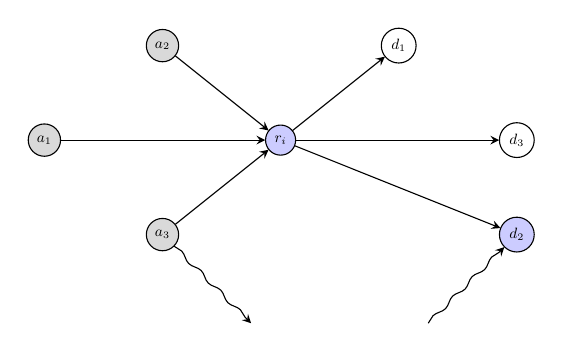
\begin{tikzpicture}[scale=.6, transform shape]
    
      % ---- ESTILOS ----
      \tikzstyle{nodo}      =[circle, draw, minimum size=18pt, font=\small] % estilo base
      \tikzstyle{visited}   =[nodo, fill=gray!30]   % ya visitado
      \tikzstyle{visiting}  =[nodo, fill=blue!20]   % en visita
      \tikzstyle{arista}    =[->, >=stealth]        % aristas
      \tikzstyle{mySnake}   =[decorate, decoration={snake, amplitude=0.7pt}] % para líneas onduladas
    
      % ---- NODOS ----
      \node[visited]  (a1)  at (0,   0) {$a_1$};
      \node[visited]  (a2)  at (2.5,  2) {$a_2$};
      \node[visited]     (a3)  at (2.5, -2) {$a_3$};
      \node[visiting] (xi)  at (5,   0) {$r_i$};
      \node[nodo]  (d_1) at (7.5, 2) {$d_1$};
      \node[visiting]     (d_2) at (10, -2) {$d_2$};
      \node[nodo]     (d_3) at (10,  0) {$d_3$};
    
      % nodos “fantasma” para las líneas onduladas
      \node[draw=none, fill=none] (hijo_a3) at (4.5, -4) {};
      \node[draw=none, fill=none] (hijo_d2) at (8,   -4) {};
    
      % ---- ARISTAS ----
      \path (a1) edge[arista] (xi);
      \path (a2) edge[arista] (xi);
      \path (a3) edge[arista] (xi);
    
      \path (xi) edge[arista] (d_1);
      \path (xi) edge[arista] (d_2);
      \path (xi) edge[arista] (d_3);
    
      \path (a3)      edge[arista, mySnake] node[above right] {} (hijo_a3);
      \path (hijo_d2) edge[arista, mySnake] node[below right] {} (d_2);
    
    \end{tikzpicture}
\caption{DFS enraizado en \(r_i\): los nodos grises ya fueron visitados; los azules está en proceso y los blancos no fueron procesados todavía.}
\label{fig:dfsTopoSorts}
\end{figure}

Una vez que definimos $combineNodesOrder$, nuestro algoritmo final consiste en hacer $DFS$, combinando los resultados de los vecinos no visitados. En \texttt{unifyNeighboursResults} hacemos lo mismo que en $combineNodesOrder$, unificando las tuplas con la misma posición. De este modo, presentamos la versión final del Algoritmo \ref{alg:numberToposortsPolytree}: 

\begin{algorithm}
\caption{Final - Número de órdenes topológicos para polytrees} \label{alg:numberToposortsPolytree}
\begin{algorithmic}[1]
\Function{polytreeTopsorts}{$D, node$}
    \State $topos \gets$ $\set{}$

    \If{$|unvisitedNeighbors(node,D)| = 0$}
            \State \Return $\{(0,1)\}$ %\Comment{caso base: sin vecinos no visitados}
    \EndIf
    
    \For{$order \in allNVNeighbourOrders(D, node)$}
        \State $topos \gets$ $topos \ \cup$ \Call{combineNodesOrder}{$node, order , polytree$}
    \EndFor

    \State $toposPositions \gets$ \Call{unifyNeighboursResults}{$topos$}
    \State \Return $toposPositions$
\EndFunction
\end{algorithmic}
\end{algorithm}
 

\subsection{Complejidad del algoritmo}
\label{subSection:polytreeCountingComplexity}

Vamos a analizar la complejidad del Algoritmo \ref{alg:numberToposortsPolytree}. Para eso veamos cuál es el costo de procesar cada uno de los nodos y cuántas veces vamos a llamar a esta función por cada nodo. 

Vamos a evaluar cuánto cuesta el llamado en base a $node$ y $D$. Obtener $allNVNeighbourOrders(D,node)$ va a costar $O(d_{out}(v)! \cdot d_{in}(v)!)$, pues ese es el número de todas las permutaciones posibles. Sean $v_1, \cdots, v_k$ los $k$ vecinos de $node$ y $\subtree_1, \cdots, \subtree_k$ sus subárboles visitados, con $\subtree_{max}$ el subárbol de tamaño máximo. Entonces se cumple que $|positionInTopsorts(v_i, \subtree_i)| \leq |\subtree_i| \leq |\subtree_{max}|$, pues las posiciones en las que puede estar un nodo en un orden topológico están acotadas por la longitud del orden. Así que en $combineNodesOrder$ se realiza la unión de $O(|\subtree_{max}|^k)$ elementos. 

Por último tenemos la complejidad de llamar a $posAndOrd$, la cual depende de la complejidad de $allPosibleOrders$. El cálculo de esta complejidad se encuentra en la sección \ref{subsubSection:allPosibleOrdersComplexity} del apéndice, pero para un grado de vecinos $k$ acotado, se llega a la cota $O(n^{3k-1})$ para su complejidad. 

Así nuestra complejidad final nos queda $O(allNVNeighbourOrders) \cdot O(combineNodesOrder) \cdot O(allPosibleOrders)$, siendo $k$ nuestro grado acotado para los vecinos. Así la complejidad total nos queda $O(k! \cdot n^k \cdot  n^{3k-1}) = O(k! n^{4k-1})$, para nuestro algoritmo de conteo completo. 



%\echu{También creo que sería mandar la complejidad del allPosibleOrders al apéndice y acá sólo poner que esa es la complejidad y que me crean, o que me elijan creer.} Rta: Sup, juega esa

%\echu{No se entiende nada metiendo pit o pot, ver como hacer que se entienda. De última meter los nombres completos y lesto}

%TODO: Escribir esta complejidad, en base a la función:
%def allPossibleOrders(nodeIndex : i, nodesBefore : list[int] , nodesAfter : list[int], lastNode : int, nodesToPutBefore : int, placedNodeIndex: int) -> int:
%placedNodeIndex y lastNode son constantes
%Se que los dos primeros parametros los puedo acotar por |st_max|^|order| (pues son listas de order elementos), y los otros párametros los puedo acotar por n (nodos totales).
%Ahí me va a quedar polinomial, si el grafo es acotado ¿Es suficientemente fina la cota o queremos hacer algo mejor y más exacto?
